%File: main.tex -- *ACL format (acl-org/acl-style-files). Human input-error perturbations paper.
% Layout follows the attention-sink paper: finding boxes (hypbox), \paragraph{Method.} blocks,
% claim-first results paragraphs. All numbers marked \todo are placeholders to be measured.
\documentclass[11pt]{article}

% "review" for anonymous submission with line numbers; change to "final" for camera-ready.
\usepackage[review]{acl}

% Standard package includes per the ACL template
\usepackage{times}
\usepackage{latexsym}
\usepackage[T1]{fontenc}
\usepackage[utf8]{inputenc}
\usepackage{microtype}
\usepackage{graphicx}

% acl.sty already loads natbib, caption, hyperref, and geometry
\usepackage{amsmath}
\usepackage{amssymb}
\usepackage{booktabs}
\usepackage{multirow}
\usepackage{enumitem}
\usepackage{xcolor}
\usepackage{tcolorbox}
\newtcolorbox{hypbox}{colback=gray!8,colframe=gray!45,boxrule=0.5pt,arc=2pt,left=5pt,right=5pt,top=3pt,bottom=3pt}
\newcommand{\todo}[1]{\textcolor{red}{[#1]}}
\newtcolorbox{modbox}{colback=white,colframe=gray!55,boxrule=0.4pt,arc=1.5pt,left=4pt,right=4pt,top=2pt,bottom=2pt}
\setcounter{secnumdepth}{2}

\title{Measuring and Mitigating Human Input-Error Perturbations in Language Models}
\author{Zizhao Hu \\
  Department of Computer Science, University of Southern California \\
  \texttt{zizhaohu@usc.edu}}

\begin{document}
\maketitle

\begin{abstract}
Language models are evaluated on clean text, but humans do not produce clean text: keyboards slip
and speech recognizers mishear. We collect a perturbation methodology set that models human input
errors in their three modalities, keyboard, voice, and copy--paste, and use it both to evaluate
models under realistic input noise and to augment training data with the same noise. Applying the
set at matched perturbation rates separates the modalities: keyboard errors, which are local and
character-level, degrade model performance far less than voice errors, which substitute and merge
whole words and so change what the input says; copy--paste errors drop, duplicate, or import whole
spans and sit between the two \todo{confirm ordering once measured}. Building on this split, we propose a mitigation
that \todo{one-line method description}, recovering \todo{XX} of the perturbed-input loss while
leaving clean-input performance unchanged. Input-error robustness is a modality property, not a
noise-rate property, and it can be trained for.
\end{abstract}

\section{Introduction}
A deployed language model never sees the text its user intended. Between intention and input sit
three noisy channels: the keyboard, where fingers hit adjacent keys, transpose characters, and
drop letters; the microphone, where a speech recognizer substitutes homophones, merges words, and
deletes the punctuation that structure depends on; and the clipboard, where a selection misses its
edge words, pastes twice, or carries formatting debris from its source. Benchmarks score models on the intended text;
users experience models on the transmitted text. The gap between the two is the subject of this
paper.

The two channels corrupt text in structurally different ways. A keyboard error is local: it
changes characters inside a word, usually leaving the word recoverable from its neighbors and its
shape. A voice error is global: it replaces the word with a different real word, or re-segments a
span entirely, so the corrupted input is fluent text that says something else. If models read
through local corruption but are misled by fluent corruption, then robustness to human input error
is a property of the input modality, not of the noise rate, and evaluation and mitigation should
be organized by modality.

We make three contributions:
\begin{enumerate}[label=\arabic*.,leftmargin=1.35em,topsep=1pt,itemsep=1pt,parsep=0pt,partopsep=0pt]
\item We collect a \textbf{perturbation methodology set} that models human input errors from the
keyboard, voice, and copy--paste modalities, usable both for evaluation under realistic noise and for training
data augmentation (Sec.~\ref{sec:find1}).
\item We show that \textbf{keyboard errors are less harmful than voice errors} to a language model
at matched perturbation rates, and locate why: local character noise leaves meaning recoverable
while fluent word-level noise rewrites it (Sec.~\ref{sec:find2}).
\item We propose a \textbf{mitigation method} that reduces the harm of both input-error
modalities, recovering most of the perturbed-input loss without damaging clean-input performance
(Sec.~\ref{sec:method}).
\end{enumerate}

\section{Related Work}
\label{sec:related}

\paragraph{Robustness to input noise.} \todo{cite: character-level adversarial and typo robustness
work; synthetic vs natural typo studies; noise injection for NMT and classification. Fetch real
citations from arXiv before submission, no invented references.} Prior robustness work
concentrates on synthetic character noise or adversarial perturbations chosen to break the model.
Human input errors differ on both counts: they are natural, high-frequency, and modality-shaped,
and they arrive at inference time whether or not an adversary exists.

\paragraph{Speech-channel errors.} \todo{cite: ASR error analysis, homophone confusion, cascaded
spoken-language-understanding robustness.} Cascaded systems that feed recognizer output into a
language model inherit the recognizer's confusions, which are fluent by construction: the
recognizer emits real words. This places voice errors in a different class from keyboard slips,
a distinction our evaluation makes measurable.

\paragraph{Noise-aware training.} \todo{cite: data augmentation with synthetic noise, consistency
training, input normalization front-ends.} Augmentation with synthetic noise improves robustness
to that noise; the open question our method addresses is which noise to train with when the
deployed noise is modality-mixed, and whether robustness to one modality transfers to the other.

\section{Findings}

We present our findings in two sections. The first builds the perturbation methodology set and
establishes that human input errors are structured by modality (Finding~1, \S\ref{sec:find1}).
The second applies the set at matched rates and separates the modalities by the harm they cause
(Finding~2, \S\ref{sec:find2}).

\subsection{A perturbation methodology set for human input errors}
\label{sec:find1}

\begin{hypbox}
\textbf{Finding 1: human input errors are structured by modality.} Keyboard errors are local and
character-level, leaving words recoverable from shape and context; voice errors are global and
word-level, producing fluent text that says something else; copy--paste errors are structural and
span-level, dropping, duplicating, or importing whole stretches. The three modalities therefore
define three distinct perturbation families, not one noise dial.
\end{hypbox}

\begin{figure*}[t]
\centering
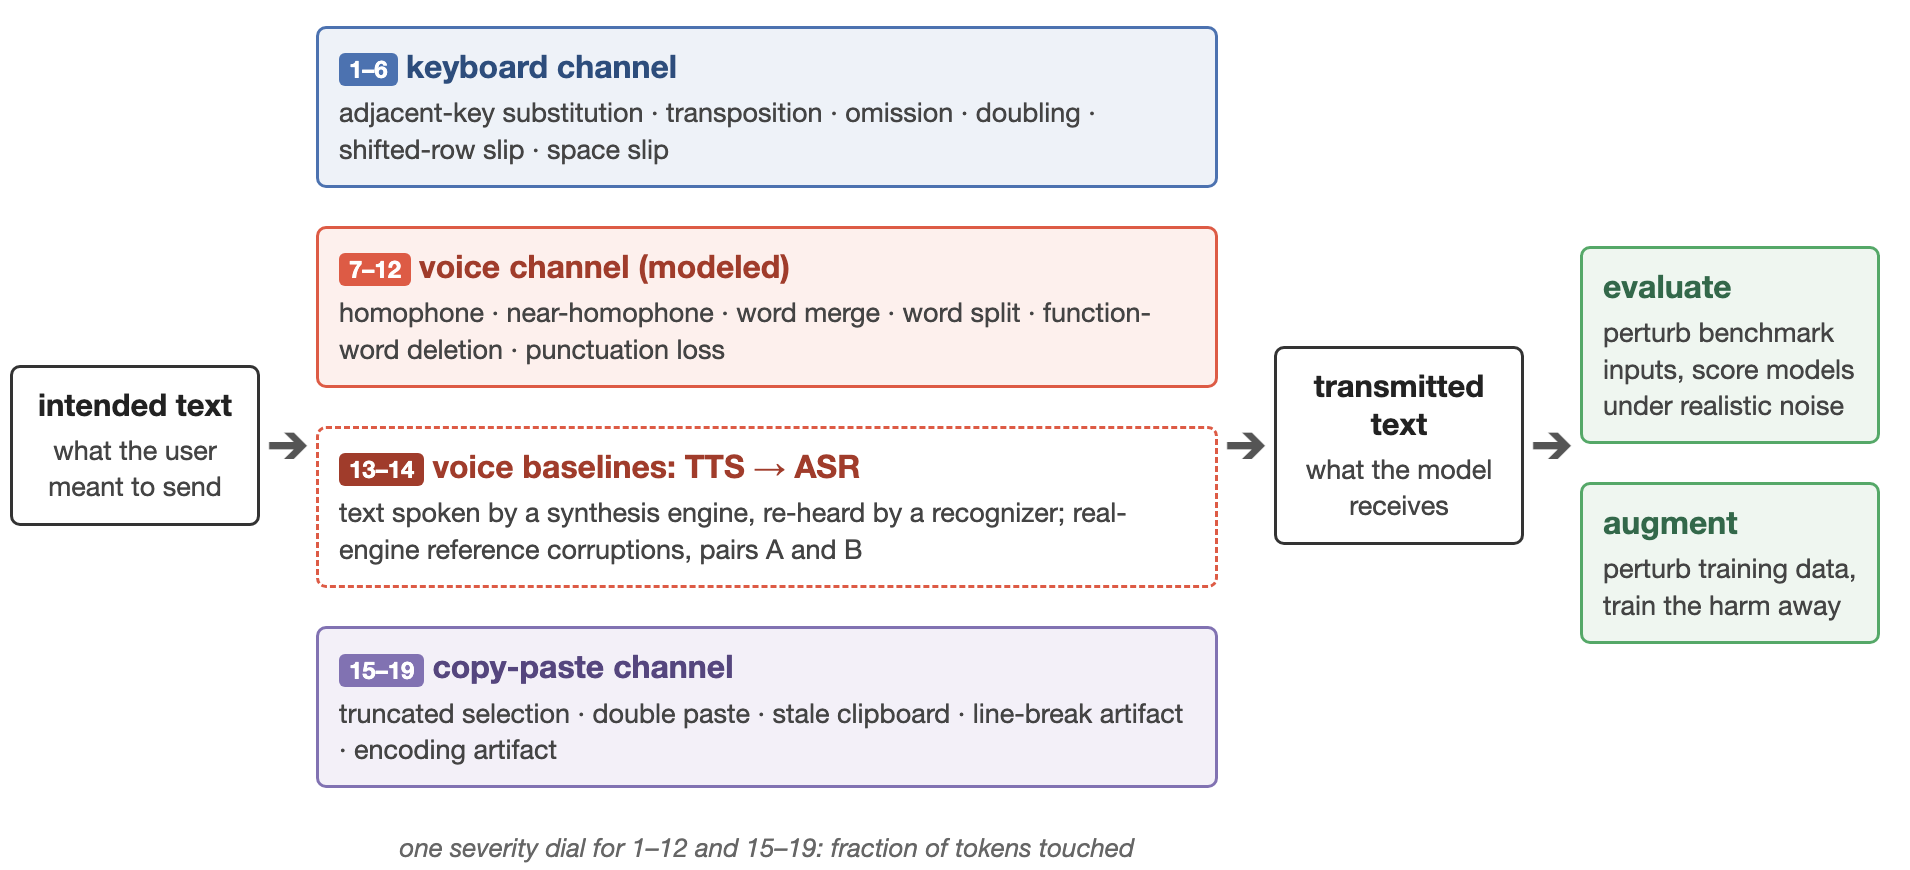
\includegraphics[width=\textwidth]{figures/pipeline.png}
\caption{The perturbation pipeline. Intended text passes through one of the modeled channels,
keyboard ($1$--$6$), voice ($7$--$12$) with its TTS$\to$ASR roundtrip baselines ($13$--$14$), or
copy--paste ($15$--$19$), and the transmitted text feeds evaluation and augmentation. The full
operator set is in Tab.~\ref{tab:operators} (App.~\ref{app:operators}).}
\label{fig:pipeline}
\end{figure*}

\paragraph{Method.} We build each family from the physical error process of its channel
(Fig.~\ref{fig:pipeline}; full set in Tab.~\ref{tab:operators}, App.~\ref{app:operators}).
Every modeled operator exposes the same severity dial, the fraction of tokens touched, so the
families can be applied at matched rates, and the set supports two uses unchanged: perturbing
benchmark inputs for evaluation, and perturbing training data for augmentation.

\begin{modbox}
\textbf{Keyboard (operators $1$--$6$).} Local, character-level, out-of-vocabulary by nature.
\end{modbox}

Keyboard operators model the hands: adjacent-key substitution weighted by key distance on the
layout, character transposition, omission, doubling, shifted-row slips, and space slips, with
per-character error rates calibrated to \todo{typing-corpus source}. The corruption stays inside
the word: the result is usually a non-word whose intended form is recoverable from shape, edit
distance, and context, which is exactly the regime spell checkers and readers repair.

\begin{modbox}
\textbf{Voice (operators $7$--$12$, baselines $13$--$14$).} Global, word-level, fluent by
construction; split into a readout stage and a transcription stage.
\end{modbox}

\emph{Readout.} The first corruption happens before any recognizer runs: the speaker's rendition
of the intended text, with disfluencies, false starts, mispronunciations, and prosody that drops
the punctuation structure writing would carry. The set captures readout error through the
synthesis half of the roundtrip baselines, which speak the text aloud before it is re-heard, and
through the punctuation-loss operator, since spoken input carries no punctuation at all
\todo{optionally add modeled disfluency operators if the readout share proves large}.

\emph{Transcription.} The recognizer then maps audio back to text and errs toward fluent
substitutes: homophone and near-homophone substitution, word merge and split, and function-word
deletion, with confusion statistics drawn from \todo{ASR confusion source}. The two TTS$\to$ASR
roundtrip baselines (operators $13$ and $14$) speak the text through a synthesis engine and
re-hear it with a recognizer, giving reference corruptions from real engine pairs that bundle
readout and transcription error as deployment does.

\begin{modbox}
\textbf{Copy--paste (operators $15$--$19$).} Structural, span-level; the text is exact where it
survives and wrong in blocks where it does not.
\end{modbox}

Copy--paste operators model the clipboard: truncated selection that misses edge words, double
paste, stale clipboard content replacing the intended text, and the formatting debris of the
source, retained line breaks with hyphenation and mis-decoded quotes and spaces, with rates
calibrated to \todo{clipboard/log source}. Unlike the other channels the corruption is not noisy
per token: spans are perfectly right or wholly wrong, missing, or foreign.

\paragraph{The families do not overlap.} Applied to the same text at the same rate, the families
produce measurably different corruptions: keyboard operators leave \todo{XX\%} of perturbed words
out-of-vocabulary and recoverable by edit distance \todo{$\le k$}; voice operators leave
\todo{XX\%} of perturbed words as valid vocabulary items, invisible to a spell checker by
construction; copy--paste operators leave individual words intact \todo{XX\%} of the time while
changing span length by \todo{measure}. \todo{One quantitative divergence measure between the
families, e.g. distribution over edit types.} A single noise rate therefore under-specifies the
perturbation; the modality is the load-bearing variable.

\paragraph{What the receiver does with a corrupted input.} Harm depends on the receiver as much
as the channel, so we fix the response taxonomy before measuring.

\begin{modbox}
\textbf{In the human.} A human reader repairs, asks, or stalls, and almost never answers the
corrupted question as written.
\end{modbox}

Human receivers resolve most keyboard corruption silently, reading through non-words by shape and
context; where the input is fluent but wrong, they ask back or hesitate, using the dialogue to
recover the intention rather than committing to the transmitted text \todo{cite reading-repair
and clarification-request literature; optionally a small human baseline on the same perturbed
inputs}.

\begin{modbox}
\textbf{In the LLM.} A model has the same four options but different defaults; we name and count
them.
\end{modbox}

We label every response to a perturbed input with one of four modes.
\textbf{Clarify}: the model asks back, ``did you mean \ldots?'', surfacing the corruption and
recovering the intention at the cost of a turn.
\textbf{Abstain}: the model declines, ``I don't understand'', safe but unhelpful.
\textbf{Derail}: the model proceeds confidently to a wrong answer to the intended question, the
corruption silently degrading the computation.
\textbf{Substitute}: the model answers a different question, the one the corrupted text literally
asks, fluent, self-consistent, and not what the user wanted.
Clarify and Abstain are visible failures that cost latency; Derail and Substitute are silent
failures that cost correctness, and \todo{XX\%} of voice-perturbed errors are silent against
\todo{XX\%} for keyboard \todo{measure; hypothesis: fluent corruption shifts the mix from
Clarify toward Substitute because nothing looks wrong to the model}.

\subsection{Keyboard errors harm less than voice errors}
\label{sec:find2}

\begin{hypbox}
\textbf{Finding 2: keyboard errors are less harmful than voice errors.} At matched perturbation
rates, keyboard noise costs a language model a fraction of the performance that voice noise
costs, across tasks and rates. The harm tracks whether the corruption preserves recoverable
meaning, not how many tokens it touches.
\end{hypbox}

% figure placeholder: harm curves, task metric vs perturbation rate, one line per modality
% \noindent\begin{minipage}{\linewidth}\centering
% \includegraphics[width=\linewidth]{figures/harm_curves.png}
% \captionof{figure}{Task performance against perturbation rate. Left: \todo{task A}. Right:
% \todo{task B}. Keyboard degrades gently; voice degrades steeply at the same rate.}
% \label{fig:harm}
% \end{minipage}\par\medskip

\paragraph{Method.} We apply both families to the inputs of \todo{benchmark list} at rates
\todo{sweep, e.g. 2 to 30 percent of tokens} and score \todo{model list} zero-shot, holding
prompts, decoding, and metrics fixed so only the input perturbation varies; each response is also
labeled with the four-mode taxonomy of \S\ref{sec:find1}. Clean-input scores anchor each curve.
\todo{n, seeds, SEM protocol.}

\paragraph{Voice noise costs a multiple of keyboard noise.} At a matched \todo{X\%} rate,
keyboard perturbation moves \todo{task metric} from \todo{clean} to \todo{value}, while voice
perturbation moves it to \todo{value}, a \todo{Y$\times$} larger drop; the gap widens with rate.
\todo{One sentence on which voice operators drive the harm, e.g. homophone substitution versus
punctuation loss, from the per-operator ablation.} The model reads through what a human reader
reads through, and is misled where a human would need the audio.

\section{Reducing the harm}
\label{sec:method}

\paragraph{Method.} \todo{The mitigation. Candidate framing to fill in once measured: train-time
augmentation with the modality-matched perturbation set at a mixing ratio, optionally paired with
an input-normalization step; state the training recipe, budget, and the clean-input control.}

\paragraph{The mitigation recovers most of the perturbed-input loss.} \todo{Headline numbers:
perturbed-input metric before and after mitigation per modality, clean-input metric unchanged
within noise, transfer between modalities.} \todo{One sentence on the asymmetry: whether
keyboard-trained robustness transfers to voice, and the cheaper direction.}

\paragraph{Limitations.} \todo{Bound the claims once results land: models and tasks covered,
calibration sources for the error statistics, synthetic-versus-logged human error gap, and any
imputed cells, disclosed.}

\section{Conclusion}
Human input errors are not one noise source but three: the keyboard corrupts characters and
leaves meaning recoverable, the voice channel corrupts words and rewrites meaning, the clipboard
corrupts spans wholesale, and a language model inherits exactly that structure, robust where
recovery is possible and fragile where the input is fluent but wrong. The perturbation set makes the asymmetry measurable and trainable:
\todo{one-sentence summary of the mitigation result}. Evaluation under clean text overstates
robustness for voice-facing deployments, and the fix is to state robustness per modality.

\raggedbottom
% \bibliography{references}  % re-enable once verified entries are added; an empty bib breaks the build

\appendix

\section{The perturbation operator set}
\label{app:operators}

Tab.~\ref{tab:operators} lists the full set: the twelve modeled operators with the physical
error each models and a worked example, and the two TTS$\to$ASR roundtrip baselines.

% The full perturbation operator set. Operators 1-12 are the modeled keyboard and voice
% families, 13-14 the TTS->ASR roundtrip baselines, 15-19 the modeled copy-paste family.
\begin{table*}[t]
\centering
\scriptsize
\setlength{\tabcolsep}{4pt}
\begin{tabular*}{\textwidth}{@{\extracolsep{\fill}} r l l l l}
\toprule
\# & family & operator & models & example (\emph{the road is clear}) \\
\midrule
1 & keyboard & adjacent-key substitution & finger lands on a neighboring key & the roas is clear\\
2 & keyboard & transposition & two keystrokes swap order & the raod is clear\\
3 & keyboard & omission & keystroke missed & the rad is clear\\
4 & keyboard & doubling & key registers twice & the rooad is clear\\
5 & keyboard & shifted-row slip & hand offset by one row & the 4oad is clear\\
6 & keyboard & space slip & space dropped or inserted & ther oad is clear\\
\midrule
7 & voice & homophone substitution & recognizer picks the homophone & the rode is clear\\
8 & voice & near-homophone substitution & acoustically close word wins & the load is clear\\
9 & voice & word merge & two words heard as one & the roadis clear\\
10 & voice & word split & one word heard as two & the row dis clear\\
11 & voice & function-word deletion & short unstressed word dropped & road is clear\\
12 & voice & punctuation loss & spoken input carries no punctuation & the road is clear no boundary\\
\midrule
13 & baseline & TTS$\to$ASR roundtrip A & real engine pair \todo{TTS A $+$ ASR A} & \todo{logged output}\\
14 & baseline & TTS$\to$ASR roundtrip B & real engine pair \todo{TTS B $+$ ASR B} & \todo{logged output}\\
\midrule
15 & copy-paste & truncated selection & selection misses edge words & road is clear\\
16 & copy-paste & double paste & clipboard pasted twice & the road is clearthe road is clear\\
17 & copy-paste & stale clipboard & previous clipboard content pasted & meeting moved to 3pm\\
18 & copy-paste & line-break artifact & PDF hyphenation and breaks retained & the ro- ad is clear\\
19 & copy-paste & encoding artifact & quotes and spaces mis-decoded & the road is clear\\
\bottomrule
\end{tabular*}
\caption{The perturbation operator set: operators $1$--$12$ and $15$--$19$ are the modeled
methodology set, each with the same severity dial; operators $13$--$14$ are TTS$\to$ASR
roundtrip baselines that produce reference voice corruptions through real engines.}
\label{tab:operators}
\end{table*}


\end{document}
